\chapter{Contexte : un besoin d'explicabilité}
Expliquer les modèles de décisions boites noires est un besoin se faisant de plus en plus ressentir et suscitant de nombreux débats et tables rondes dans la communauté scientifique. Les entreprises recherchent avant toute chose la performance et ce au détriment de la transparence des algorithmes utilisés. En effet dans le domaine du machine learning il existe une multitude d'algorithmes pouvant être utilisés afin de fournir une prédiction, mais il existe une corrélation non négligeable entre les performances et la transparence de notre modèle comme le montre la figure \ref{performanceAndInterpretabilite}. En général, plus notre modèle est performant, plus il est difficile à comprendre.\par

\begin{figure}[h]
\centering
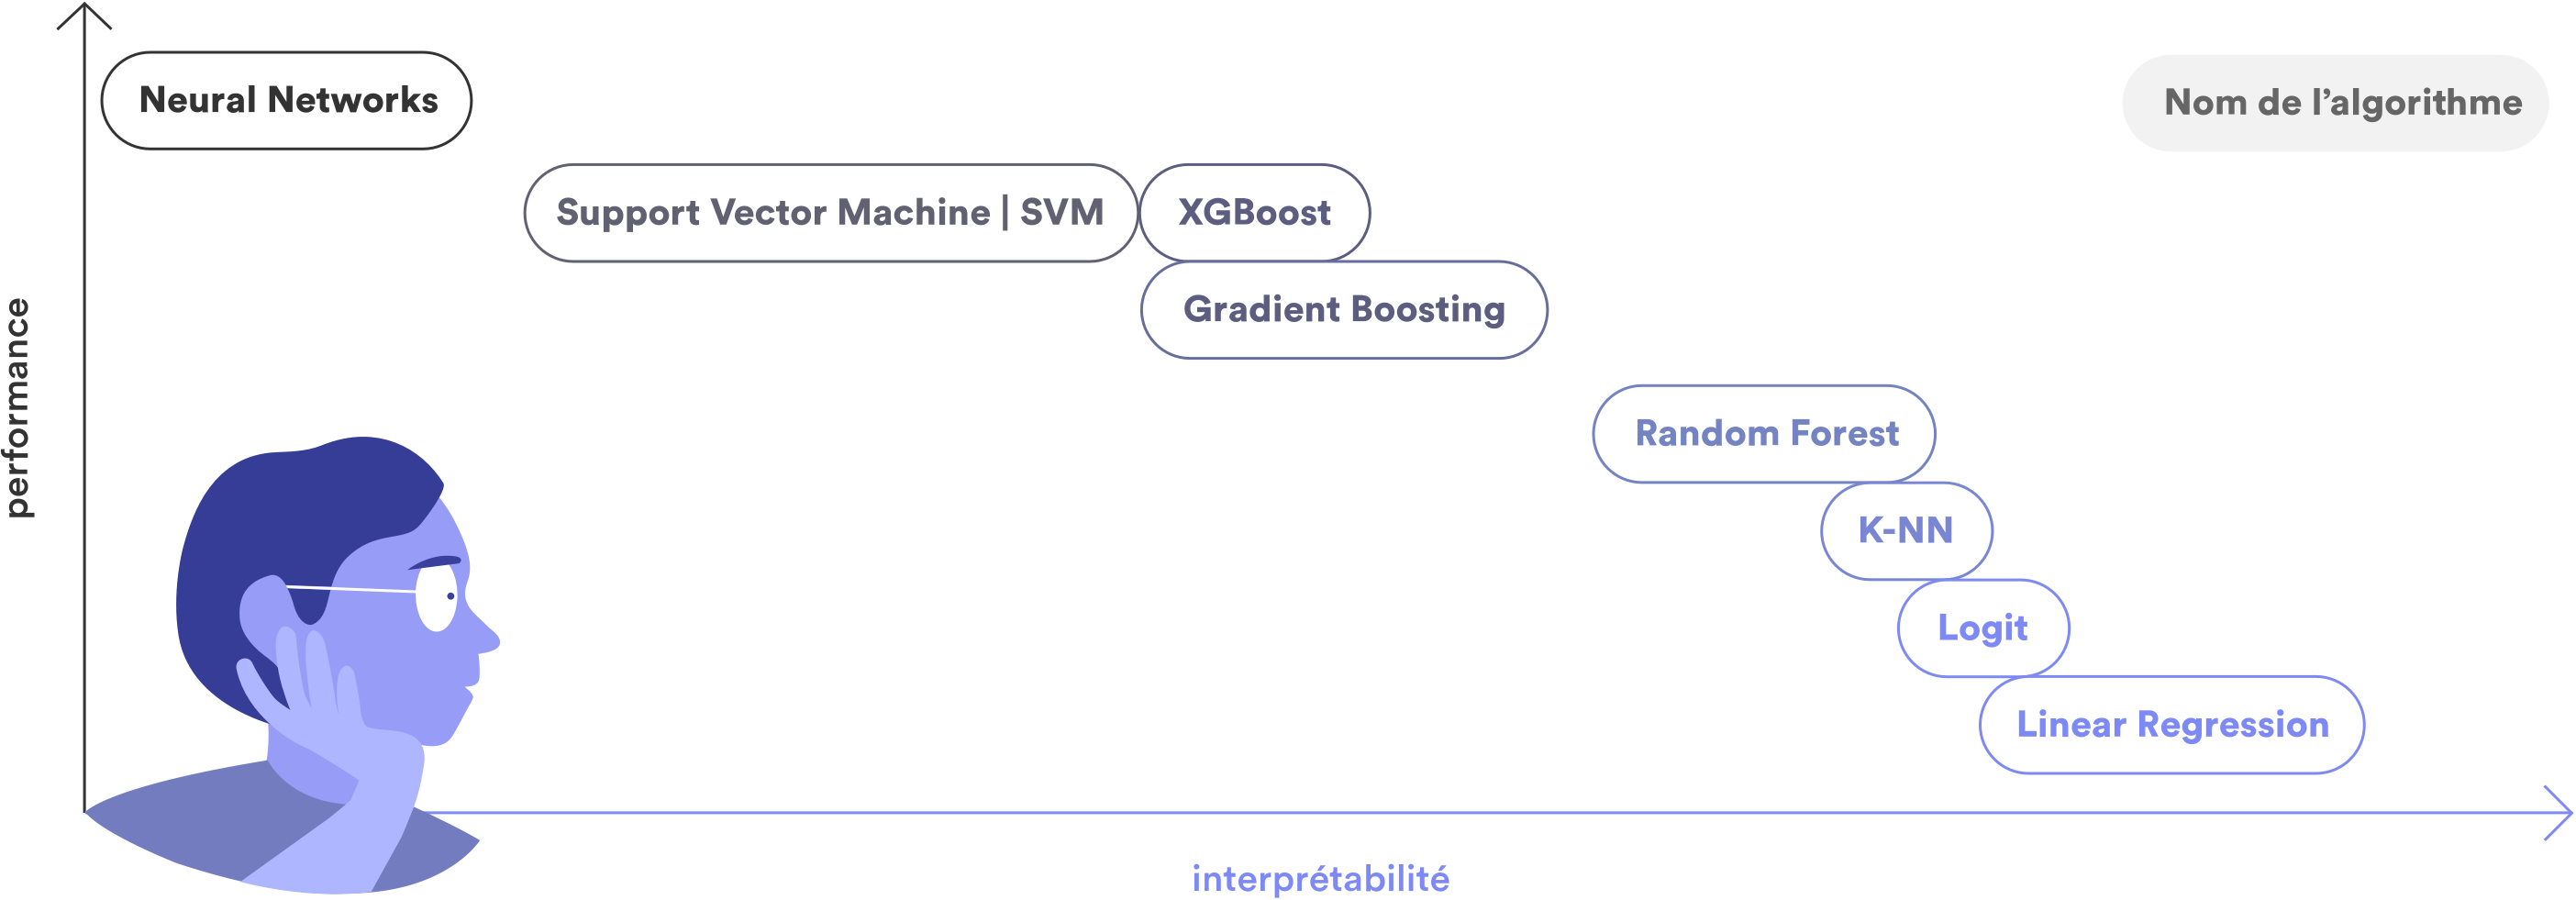
\includegraphics[scale=0.15]{src_img/performanceAndInterpretabilite.png}
\caption{Lien entre la performance et l'interprétabilité d'un algorithme de machine learning. \textit{Source \cite{hippocrate}}}
\label{performanceAndInterpretabilite}
\end{figure}

À l'heure actuelle, le réseau de neurones artificiel fait partie des algorithmes les plus performante et aussi est le plus couramment utilisée.
La non-explicabilité de ces modèles posent des problèmes de fiabilité, d'éthique et de responsabilité. Ce floue accentue aussi la méfiance et la peur des personnes envers l'intelligence artificielle, et entraîne un problème de compréhension entre les Data Scientist et les expert métier qui en plus de ne pas comprendre comment fonctionne le modèle ne comprennent pas non plus son résultat. Aussi, expliquer ces modèles permettrai d'améliorer notre conformité à la loi ainsi que d'augmenter les performances de nos modèles. Cette nouvelle problématique présente donc de nombreux enjeux de tailles.\par

\section{L'éthique}
Tout d'abord, de nombreux cas très exposés dans les médias nous montrent que cette incompréhension peut amener à des problèmes du point de vue éthique. La question de l'éthique est souvent ramenée à deux aspects principaux : la discrimination et la protection des données privées des usagers.
\subsection{La discrimination}
La question essentielle à se poser est de savoir comment une intelligence artificielle est amenée à prendre des décisions discriminante. Dans un article, Barocas et Selbst distinguent cinq façons par lesquelles une intelligence artificielle pourrait aboutir à une discrimination \cite{discriminationWay}. Ces cas sont uniquement des cas involontaires et ne prennent pas en compte une discrimination délibérée qui pourrait bien évidemment être possible.
\begin{itemize}
    \item \textbf{Définition des variables cibles et des étiquettes de classes} : le but d'une intelligence artificielle est de découvrir des corrélations dans des jeux de données. Ainsi, certain choix de variables cibles ou d'étiquettes de classes peuvent amener à faire des corrélations discriminatoire. Un exemple trivial serait de considérer un modèle permettant de savoir si un employé fait du travail de qualité, l'entreprise choisira de prendre en compte les retards des employés dans son modèle d'évaluation. Les personnes défavorisées habitant souvent loin de leur lieu de travail, ont plus souvent tendance à être en retard à cause des embouteillages et des problèmes de transport. Ces employés habitant loin, seront jugés comme faisant du travail de moins bonne qualité ce qui n'est pas forcément le cas. Si on ajoute à cela le fait que les personnes issus de l'immigration sont en moyenne plus pauvre et habitent en moyenne plus loin des centres villes, nous pouvons arriver involontairement à une IA discriminante par le simple fait d'utiliser l'étiquette "retard" dans l'évaluation des performances d'un employé.
    \item \textbf{Les données d'apprentissage} : les données d'apprentissage peuvent contenir des biais qui seront ensuite appris par notre modèle. L'exemple de l'IA de recrutement de l'entreprise Amazon qui rejetait les CVs contenant le mot "femme"\cite{amazonAi} évoqué en introduction le montre bien. Cette IA avait enfaîte appris en analysant tous les profils recrutés par Amzon dans le passé, or les personnes recrutées étaient dans l'ensemble majoritairement des hommes et très majoritairement pour les postes technique. L'IA a donc déduis qu'il était préférable de recruter des hommes.
    \item \textbf{La collecte des données d'apprentissages} : Les lieux dans lesquels sont récoltées les données d'apprentissage sont aussi déterminant. Par exemple si l'on récolte des données concernant la criminalité dans un quartier avec des personnes issus majoritairement de l'immigration, l'IA aura plus tendance à considérer les immigrés comme de potentiels criminels par rapport aux personnes non-imigrées et inversement si on choisis un quartier avec des personnes majoritairement non-imigrées.
    \item \textbf{La sélection des caractéristiques} : Afin que l'IA puisse s'entraîner, il faut lui fournir des données qui sont en réalité une représentation simplifiée de notre monde. Ainsi, son créateur doit faire des choix pour sélectionner les caractéristiques qui constitueront cette représentation. Ce choix peut par concours de circonstance involontairement découler sur de la discrimination il faut donc les choisir avec parcimonie.
    \item \textbf{Données indirect} : Certaines données peuvent inclure des données indirect. Par exemple : \textit{"un jeu de données qui ne contient pas de données explicites sur l’orientation sexuelle peut tout de même la dévoiler. Une étude de 2009 a montré que les liens d’"amis" sur Facebook révèlent par une méthode de prédiction précise de l’orientation sexuelle des utilisateurs de Facebook fondée sur l’analyse de leurs liens. Le pourcentage d’"amis" s’identifiant comme homosexuels serait fortement corrélé avec l’orientation sexuelle de l’utilisateur concerné"}\cite{dicriminationAlgo}.
\end{itemize}
Mieux comprendre le fonctionnement de nos algorithmes permettrait donc de mieux se prémunir des discriminations involontaires. Aussi on pourrait prendre en compte l'explication en plus de la prédiction afin de fournir un résultat optimal. Par exemple, aux États-Unis, un algorithme appelé Compas est utilisé par les juges pour évaluer la probabilité pour un prévenu de se faire arrêter à nouveau dans les deux ans à venir. Cet algorithme est beaucoup remis en cause, car il est jugé "non-pertinant" et "discriminatoire" par certaines personnes alors que d'autres ont grandement confiance en lui, deux camps s'affrontent donc. Dans ce cas-là, fournir une explication conjointement à la prédiction permettrai de mettre tout le monde d'accord, ainsi nous pouvons prendre en compte la prévision et déterminer si dans le cas précis elle est issue d'un jugement non-pertinant, discriminatoire ou autre.
\subsection{Protection des données}
L'apprentissage d'une intelligence artificielle requière un très grand nombre de données, parmi lesquelles peuvent se trouver des données personnelles. L'utilisation d'un modèle pourrait donc aussi nécessiter de fournir des données personnelles afin d'effectuer une prédiction. L'utilisation de ces données jugées critiques est problématique, car des restrictions et des règles de protection en découlent. Tel qu'évoqué dans l'introduction, le RGPD par l'addition de plusieurs de ses articles implique un "droit à l'explication". Ce droit a été démontré par Seth Flaxman et Bryce Goodman \cite{RGPDexplanRight}, ce qui a donc pour effet d'accentuer le besoin d'applicabilité des modèles de décision boites noires. En effet, pour le moment ce droit est inaccessible par les usagers et les entreprises éprouvent des problèmes de responsabilités.

\section{Fiabilité et confiance}
Deuxièmement, expliquer les décisions prisent par un modèle boite noire permettrai d'augmenter la fiabilité que l'on lui accorde. Le modèle peut très bien fonctionner dans la plupart des cas, mais il est possible qu'il réagisse mal dans un certain cas bien spécifique. Avec l'absence de compréhension du fonctionnement interne de notre modèle, nous pouvons ne pas prévoir ce cas spécifique qui représente un risque. Le domaine médical par exemple est en attente d'une plus grande fiabilité de ses modèles en effet, une erreur peut avoir des conséquences graves et mettre en danger des personnes. La manière classique de mesurer la fiabilité d'un modèle est de calculer sa précision (accuracy), cela consiste à diviser le nombre de prédictions corrects par le nombre de prédiction total. Cette méthode indispensable ne permet pas à elle seule une fiabilité optimal en notre modèle, admettons que nous arrivons à une précision de 100\% rien ne nous dis que dans un cas très particulier notre modèle ne nous donnera pas une prédiction fausse. La compréhension de la logique interne de notre modèle serai donc un facteur supplémentaire dans la fiabilité que l'on lui donne. \par
De plus, un soudage publié par OpinionWay\cite{opinionWay} montre que 30\% des Français ont peur d'un jugement porté par l'intelligence artificielle dans le domaine financier et 21\% dans le domaine médical. L'incompréhension de la logique interne des algorithmes décisionnels tend à accentuer la méfiance envers ces technologies. Fournir une explication permettrai d'augmenter l'acceptation de ces nouvelles technologies.

\section{Performance}
Enfin, expliquer la logique interne de la boite noire permettrai d'améliorer le développement de celle-ci, de la rendre plus compétitive et plus performante. Ces explications seront aussi utiles durant leur développement afin de comprendre pourquoi notre modèle ne fonctionne pas bien dans certains cas voir même pourquoi il ne converge pas du tout.
